\section{背景} \label{section:background}
\subsection{アドレス変換}
\subsubsection{ページング}
メモリの管理単位をページと呼び,アドレス変換の際に利用する,仮想アドレスと物理アドレスの対
応表をページテーブルと呼ぶ.通常は4096 バイトを1 ページとして1 つのマッピングでその領域を
アドレス変換することができる.
1 つのページテーブルを利用してアドレス変換を行う場合,利用しない無駄なアドレスのマッピング
まで作成されるという問題点がある.通常,プロセスが利用する領域はアドレスの一部だけであり,仮
想アドレス全体のマッピングを作成すると,ページテーブルのために無駄なメモリを使用することに
なる.

これを解決するため,多くの場合は多段ページテーブルという機構が採用されている\cite{page-table-management}.多段ページ
テーブルではアドレス変換に利用する上位ビットをいくつかに区切り,小さいページテーブルを複数
作成する.上位のページテーブルは次のページテーブルのポインタを指し,利用していないアドレスは
NULL ポインタになっている.これにより,利用しない領域に無駄なメモリを使用することを防いで
いる.このページテーブルを順番にたどってアドレス変換を行うことをページウォークと呼ぶ.

\subsubsection{TLB}
TLB(Translation Lookside Buffer) はメインメモリよりも高速なキャッシュであり,アドレス変換
の結果をTLB に保存することで,アドレス変換の高速化が可能となる.ページウォークでは,複数の
ページテーブルへのアクセスが発生し,時間がかかってしまう.そこで,一度変換したアドレスのマッ
ピングはTLB に保存しておく.プログラムの局所性により,一度アクセスされた領域は近いうちに再
度アクセスされる可能性が高いため,TLB に保存したマッピングは何度も参照される可能性が高い.
TLB はメインメモリよりも高速に読み書きができるハードウェアで,かつページウォークとは違いア
クセスも一度で済むため,TLB に保存されている結果を再利用することでアドレス変換を高速に行う
ことができる.対してTLBを使用できないTLBミスが発生した場合は複数のページテーブルに
アクセスして順番に辿っていく必要があるためアドレス変換が非常に遅くなってしまう可能性がある\cite{intel-manual}.

メモリを多く利用するアプリケーションでは,TLB ミス率が増加し,アドレス変換のオーバーヘッ
ドが大きくなる.その理由として,TLB は高速である代わりに,メインメモリよりも圧倒的に容量が
少ないことが挙げられる.単純な例として,TLB が5MB の領域をカバーしている時,使用するメモ
リサイズが10MB の場合はTLB ミス率は50\% となるが,使用するメモリサイズが100MB の場合は
TLB ミス率95\% となる.実際には参照の局所性などからこのような極端な値にはならないものの,使
用するメモリサイズとTLB サイズの差が広がるほどTLB ミス率は増加することがわかる.

\subsection{ヒュージページ}
ヒュージページとは通常よりも大きなサイズのページを利用し,一度に多くの領域をアドレス変換す
ることで,効率的なアドレス変換を行う手法である.ヒュージページを使うとTLBに保存できるページ数は同じでも,1ページのサイズが増えるため
より多くのアドレスの範囲をTLBに保存できTLBミス率を減らすことができる.また,
1ページのサイズが増えることでページテーブルの削減やページウォークの短縮といった効果も得られる.

\subsubsection{Hugetlbapges}
Hugetlbpage\cite{document-hugetlbpage}はLinux におけるヒュージページを扱う方法の1 つである.Hugetlbpage では
カーネルブート時にヒュージページ専用の領域を確保しておき,プログラム内でメモリを確保する際に
ヒュージページの利用を明示的に指定することで,ヒュージページを使うことができる.Hugetlbpage
は現在あまり利用されておらず,その理由として,実際に利用するメモリの量は事前に分からないとい
うものがある.事前に確保した領域に比べて,必要とするメモリ量が多い場合はヒュージページを割り
当てることはできなくなり,少ない場合でもヒュージページ専用で確保した領域はヒュージページにし
か使えないため,利用していない無駄なメモリが生まれるといった問題点がある.また,ユーザが明示
的にヒュージページの使用を指定しなければならないため,開発者への負担や既存のプログラムでは利
用できないといった問題点も存在する.
\subsubsection{THP}
THP(Transparent Huge page)\cite{document-thp}はLinux におけるヒュージページを扱う方法の1 つで,Linux
Kernel が自動的にヒュージページの割り当てを行うことで透過的にヒュージページを使うことができ
る.THP では必要な分だけLinux Kernel が自動でヒュージページ割り当てを行い,利用が簡単なため,
Linux ではヒュージページを割り当てる際には主にこの方法が用いられる.しかし,THP では積極的
にヒュージページを割り当てようとするため,無駄なヒュージページ割り当ての発生や,ヒュージペー
ジ昇格スレッドによってCPU を使いすぎたりと,問題点も多く存在している.

\subsection{分散処理フレームワーク}
分散処理フレームワークとは,複数のコンピュータをネットワークを繋いで処理を分散し,並列処理
を行うことで巨大なデータを効率的に処理するシステムである.代表的な分散処理フレームワークとし
て,Apache Hadoop\cite{hadoop}やApache Hive\cite{hive}, Apache Tez\cite{tez}などがある.分散処理フレームワークにおけるネットワークで繋がれた複数台
のコンピュータをクラスタと呼び,クラスタは1 台のマスターノードと,複数台のワーカーノードで
構成される.マスターノードでは主にクラスタ全体の管理を行い,実際にデータ保存したり処理を行っ
たりするのがワーカーノードとなる.

図\ref{fig:ditributed-processing-system}に分散処理フレームワークの概要図を示す.マスターノード内にあるネームノードがクラスタ
に保存されているファイルのメタデータを管理し,実際のデータはワーカーノード内のデータノード
に分散して保存されている.クライアントプログラムが起動されると,マスターノード内のリソースマ
ネージャーが各ワーカーノードにリソースを割り振り,各ノードマネージャーで処理が実行される.処
理の進捗はアプリケーションごとに存在するアプリケーションマスターが担当し,全ての処理が終了す
ると,クライアントプログラムへ結果が返却される.このように,処理を複数のコンピュータに分散す
ることでアプリケーションの実行時間の削減が可能となる.また,コンピュータを追加することでその
ままリソースを増やせるスケーラビリティやデータを複製することによる耐障害性の確保といったメ
リットも存在する.

\begin{figure}
  \centering
  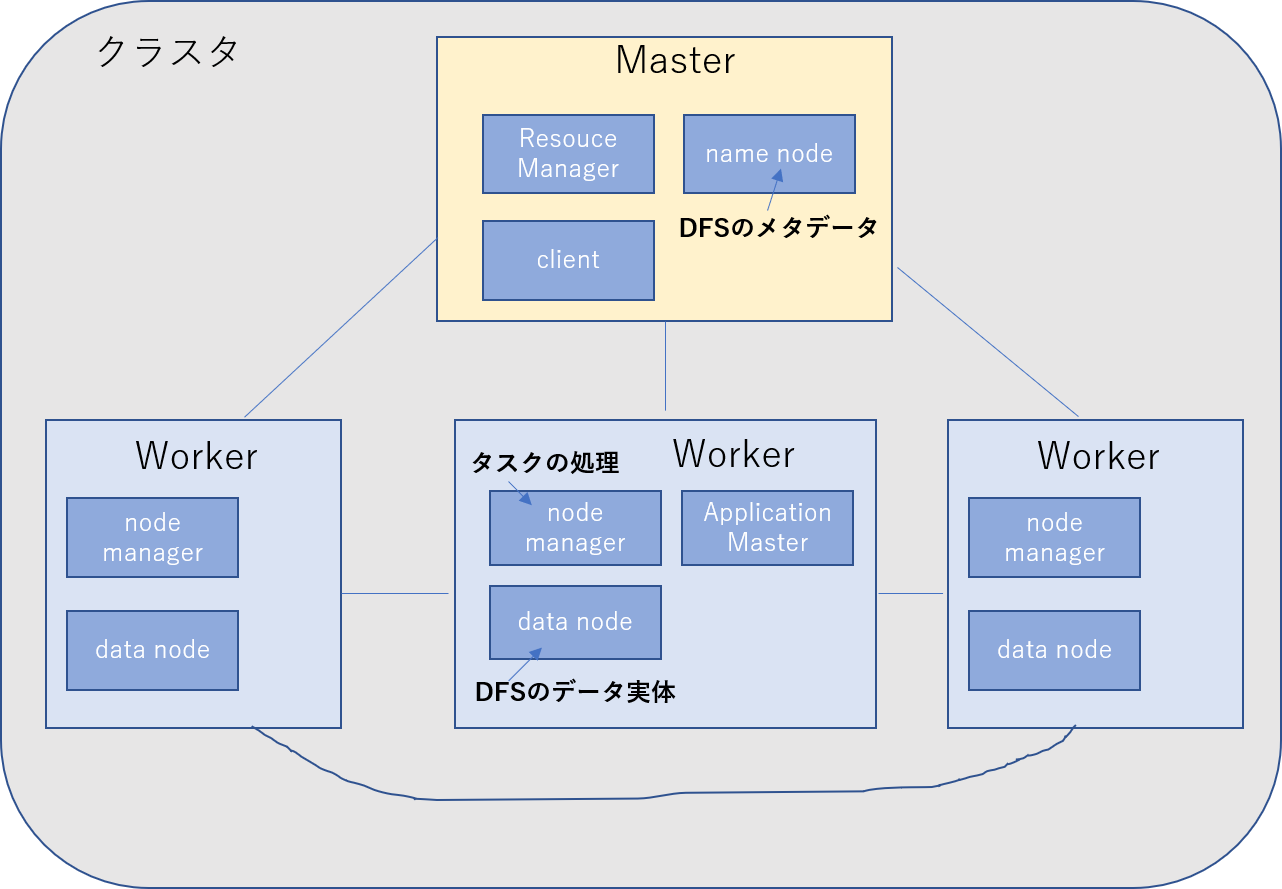
\includegraphics[scale=0.3]{figures/distributed-processing-system.png}
  \caption{分散処理フレームワーク概要図}
  \label{fig:ditributed-processing-system}
\end{figure}

\subsection{Apache Spark}
Apache Spark はインメモリ分散処理フレームワークの1 つで,分散処理フレームワークのなかでも
処理を出来る限りメモリ内で行うことでネットワークやI/O による遅延を防ぐことができる.Hadoop
などでは処理のたびにディスクアクセスが発生するため,ボトルネックが存在するという問題点がある.
Spark では処理後の一時データの出力先をディスクではなくメインメモリ
に書き出すことで,余計なディスクアクセスを減らしてHadoop の問題点を解決している.
また,ApacheSpark ではRDD\cite{zaharia2012resilient} とDAG\cite{dag} という仕組みが用いられており,処理のログを保存しておくことで,高い耐
障害性も維持している.これらのことから,分散処理フレームの中でも近年の主流となってきている.

\subsection{予備実験}
Apache Sparkへのヒュージページの効果を調査するために予備実験を行った.予備実験ではヒュージページの
割り当てをなし,全体への割り当て,StorageMemoryのみへの割り当てと3種類の状態で実験を行った.
実験結果を図\ref{fig:pre-experiment}に示す.
実験の結果ヒュージページはApache Sparkで効果的に働き実行時間を短縮させたことが分かった.また,
マイクロベンチマークやkmeansでは一部のメモリ割り当てでも全体割り当てに近い性能が得られることが分かった.
しかし,この一部割り当てを行うのはSparkからJNI\cite{jni}を通してmadviseシステムコール\cite{madvise}を呼び出すことによって,StorageMemoryのデータを
後からヒュージページに昇格していくという手法であり,ヒュージページになるのが遅く実行時間が短いと効果をあまり受けられないことや,メモリの
スキャンにオーバーヘッドがかかるという問題点が存在していた.

\begin{figure}
  \centering
  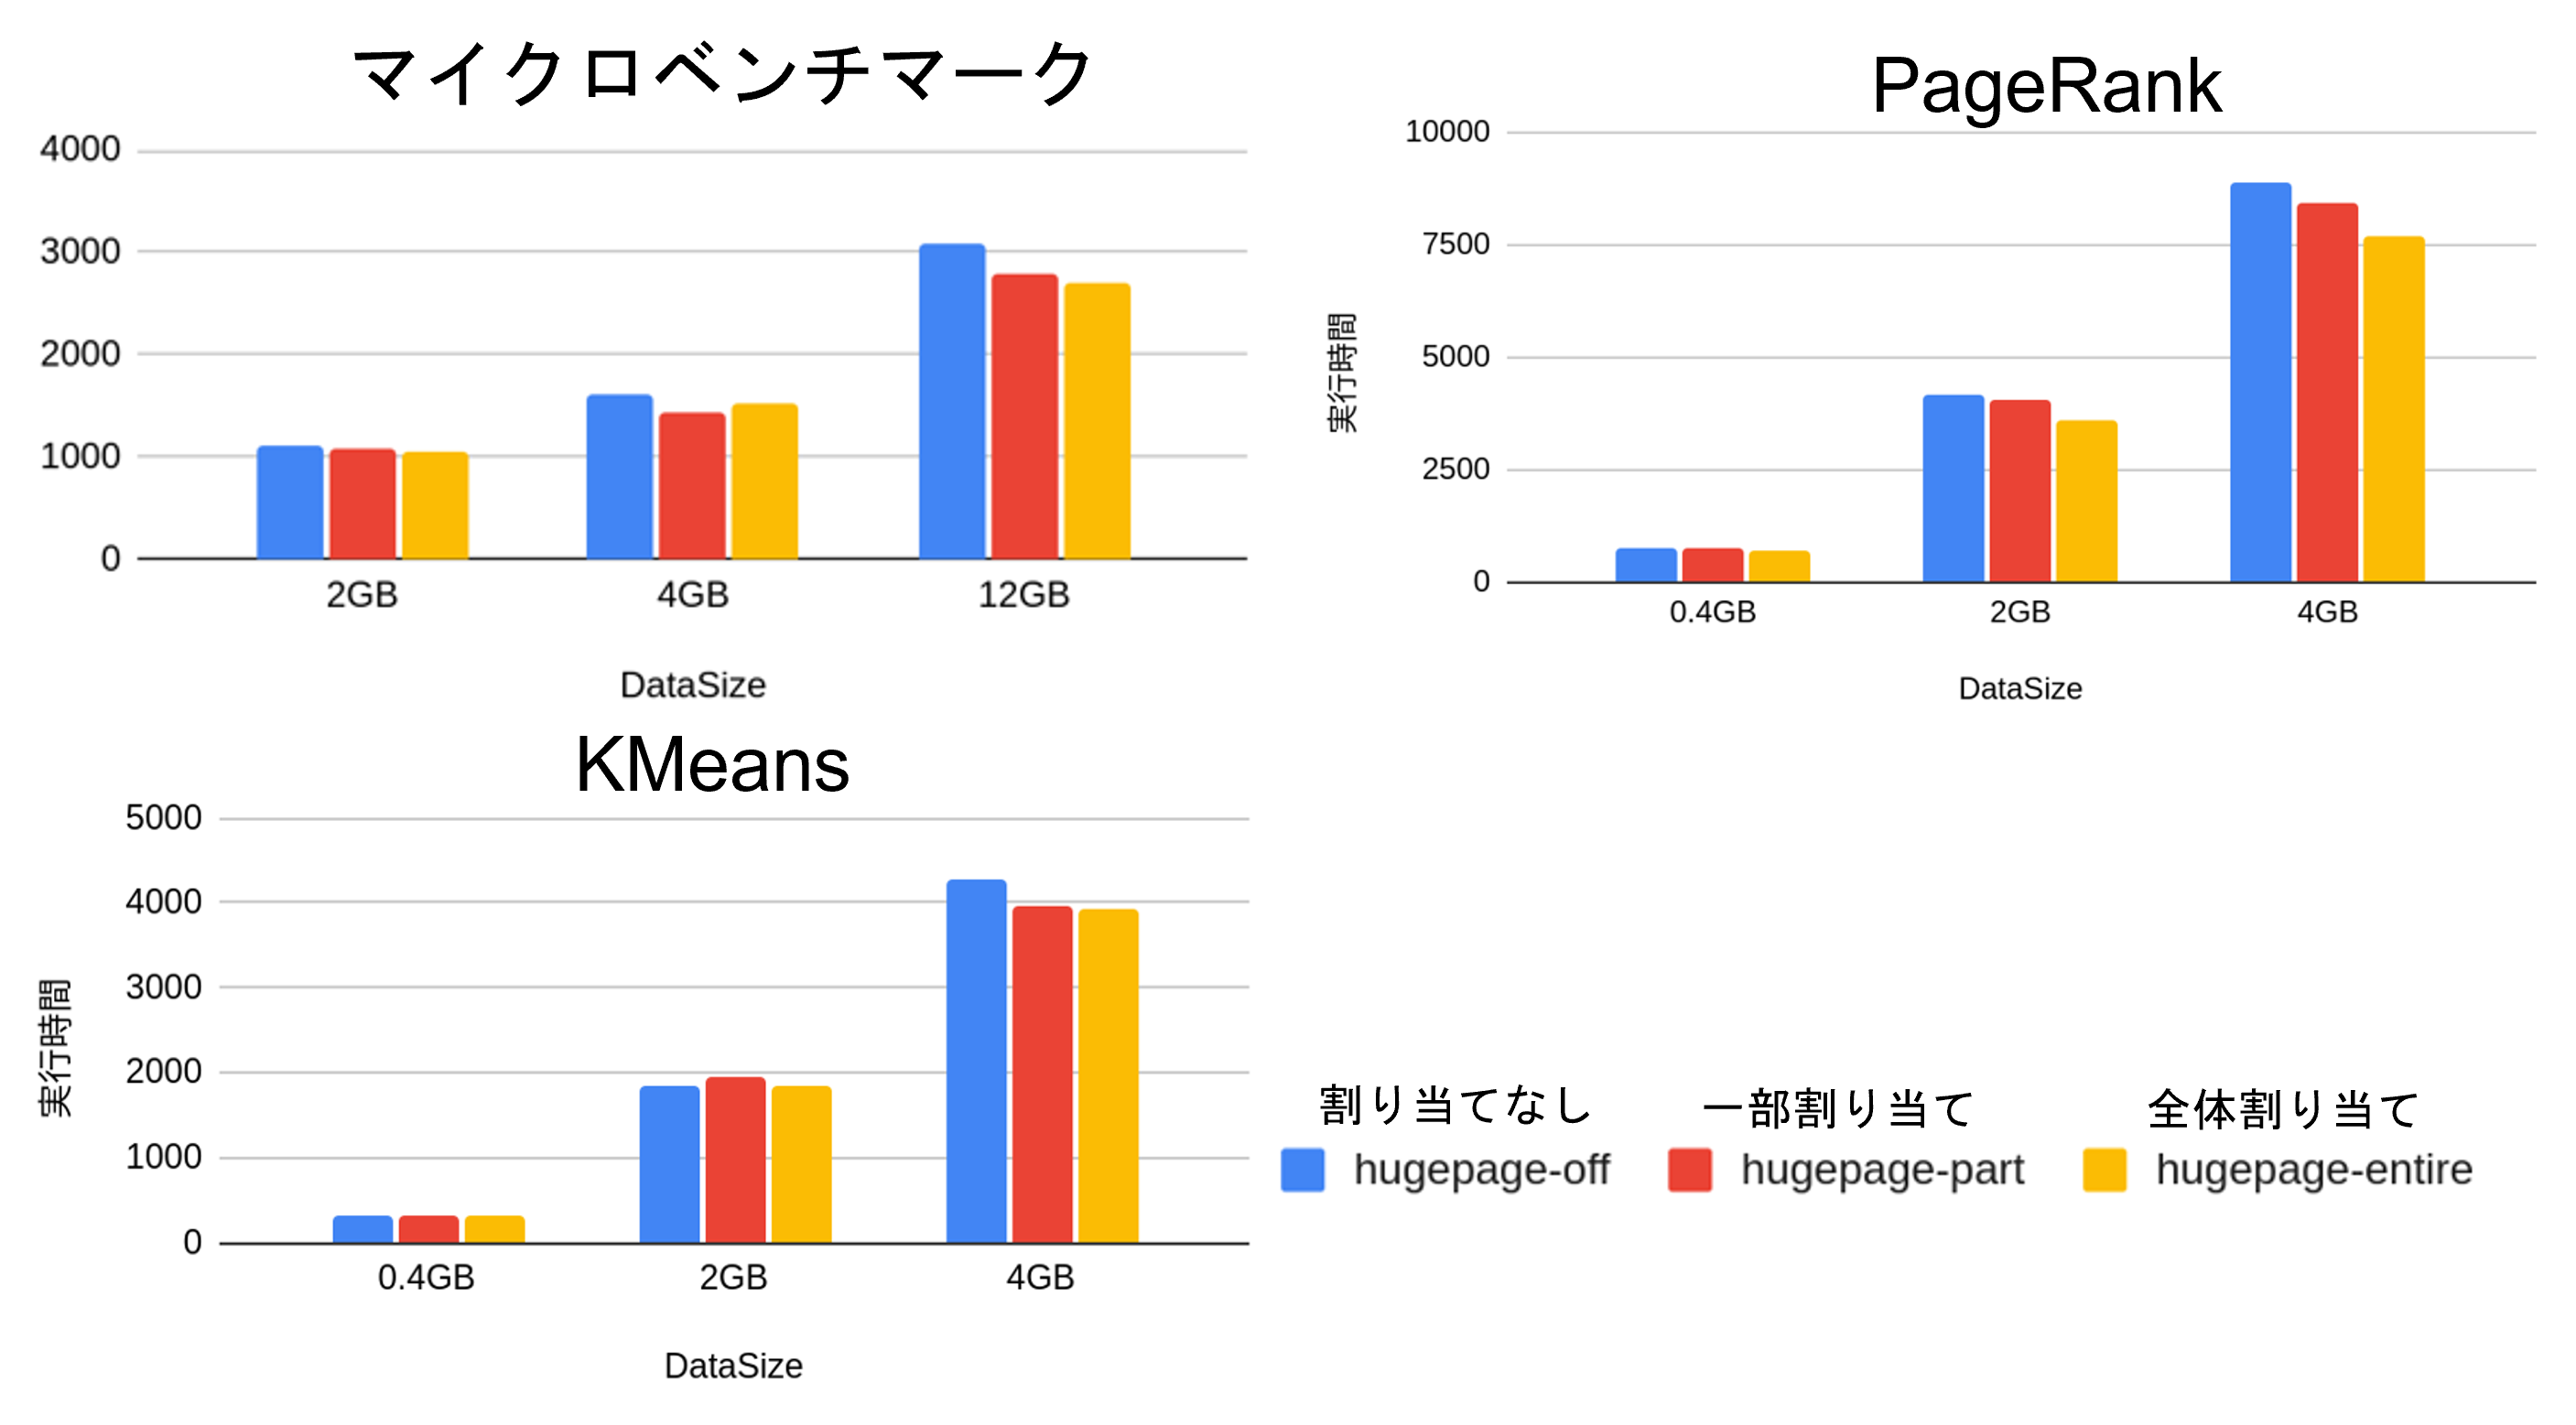
\includegraphics[scale=0.4]{figures/pre-experiment.png}
  \caption{予備実験結果}
  \label{fig:pre-experiment}
\end{figure}